\chapter{Standardabweichung des Mittelwertes}
\label{apx:meanerror}

Dieses Kapitel richtet sich leicht nach Ref.\cite{meanerrorulm}. Sei $f\equiv(f_i)$ eine Folge von $N$ Stichproben aus einer Zufallsverteilung mit einem Mittelwert $\mu$ und $\mu_N$ der empirische Mittelwert dieser Folge. Die Differenz $\Delta_N:=\mu-\mu_N$ wird nun abgeschätzt mit der Standardabweichung einer Folge von empirischen Mittelwerten $\left(\mu_{N,k}\right)$ die alle mit (sehr wahrscheinlich) verschiedenen Folgen bzw. Vektoren $(f_i)$ gebildet seien.

Sei nun $\langle \cdot \rangle_N: \mathbb{S}\times \mathbb{R}^N \rightarrow \mathbb{R}^N, \langle (f_i)_k \rangle_N:= \frac{1}{N}\sum\limits_{i=0}^N {f_i}_k$ der empirische Mittelwert und $E(\cdot):\mathbb{S}\rightarrow \mathbb{R}, E\left( x_k \right):= \lim\limits_{N\rightarrow \infty} \frac{1}{N} \sum\limits_{k=0}^N f_k$ der Erwartungswert über eine unendlich Folge aus einem beliebigen statistischen Werten für begrenzte Folgen $(f_i)$. Hierbei ist $\mathbb{S}$ der Raum der Folgen. Aus der Definition der beiden Mittelwerte wird klar, dass man die Summen und damit die Bildung der Mittelwerte vertauschen kann, sofern ein Grenzwert existiert. Dies wird in Gleichung~\ref{eq:EabToEaEb-pre} angewandt.
%\\  = \frac{1}{N} E\left( \sigma_k \right)
%    + E\left( \left( \mu_{N,k}-\mu \right)
%      \frac{1}{N} \sum\limits_{j=0,j\neq i}^N \left( f_{jk}-\mu \right) \right)
%\\  \approx \frac{1}{N} E\left( \sigma_k \right) +
%      E\left( \frac{1}{N} \sum\limits_{i=0}^N \left( f_{ik}-\mu \right)
%      \left( \mu_{N,k'} - \mu \right) \right) \\
%	= \frac{\sigma}{N} +  E\left( \left(\mu_{N,k} - \mu \right)
%	  \left( \mu_{N,k} - \mu \right) \right)
%   = \frac{\sigma}{N} +  E\left( \mu_{N,k} - \mu \right)
%	  E\left( \mu_{N,k} - \mu  \right) \\
%	= \frac{\sigma}{N} +  \left( \mu - \mu \right)\left( \mu - \mu  \right)
\begin{align}
	\sigma_{\mu_N}^2
   := E\left( \left( \mu_N - \mu \right)^2 \right)
   := E\left( \left( \langle f_{ik} \rangle_N - \mu \right)^2 \right)
	= E\left( \langle f_{ik} - \mu \rangle_N^2 \right)
\\  = E\left(
	  \left( \frac{1}{N} \sum\limits_{i=0}^N \left(f_{ik}-\mu\right) \right)
	  \left( \frac{1}{N} \sum\limits_{i=0}^N \left(f_{ik}-\mu\right) \right)
	  \right)
	= E\left( \frac{1}{N^2} \sum\limits_{i=0}^N \sum\limits_{j=0}^N
		      \left( f_{ik}-\mu \right) \left( f_{jk}-\mu \right) \right)
    \\
	\label{eq:EabToEaEb-pre}
	= \frac{1}{N} E\left(
		 \frac{1}{N} \sum\limits_{i=0}^N \left( f_{ik}-\mu \right)^2
      \right)
    + E\left( \frac{1}{N} \sum\limits_{i=0}^N \left( f_{ik}-\mu \right)
      \frac{1}{N} \sum\limits_{j=0,j\neq i}^N \left( f_{jk}-\mu \right) \right)
    \\
	\label{eq:EabToEaEb-post}
    = \frac{1}{N} E\left( \sigma_k \right)
    + \frac{1}{N} \sum\limits_{i=0}^N
      \frac{1}{N} \sum\limits_{j=0,j\neq i}^N
      \left( \underbrace{E\left(f_{ik}\right)}_{=\mu}-\mu \right)
      \left( \underbrace{E\left(f_{jk}\right)}_{=\mu}-\mu \right)
	= \uuline{ \frac{\sigma}{N} }
\end{align}
Man beachte, dass der Schritt in Gl.\ref{eq:EabToEaEb-pre}-\ref{eq:EabToEaEb-post} nur möglich ist, wenn $f_i$ unabhängig von $f_j$ ist, was hier der Fall ist, da der einzige abhängige Fall für $i=j$ aus der SUmme rausgezogen würde, sodass $E(a b)=E(a)E(b)$ anwendbar ist.

Man beachte, dass der zweite Summand nur durch die Mittelung über mehrere komplett verschiedene Versuchsreihen Null wird. Betrachtet man jedoch nur eine Versuchsreihe, dann hat der zweite Summand auch ein Skalierverhalten in Abhängigkeit zu $N$. Da aber das Vorzeichen wechseln kann, muss man den Betrag betrachten:
\begin{align}
	\frac{1}{N} \sum\limits_{i=0}^N \left( f_i-\mu \right)
    \frac{1}{N} \sum\limits_{j=0,j\neq i}^N \left( f_j-\mu \right)
    =
	\frac{1}{N} \sum\limits_{i=0}^N
    \frac{1}{N} \sum\limits_{j=0,j\neq i}^N
    \left( f_i f_j - \mu \left( f_i + f_j \right) + \mu^2 \right)
    \\
    \label{eq:approxmuN}
    \approx
	\mu_N^2 - 2 \mu \mu_N + \mu^2
	\overset{ \mu_N \approx \mu - \sigma_{\mu_N} }{\approx}
	\mu^2 - 2 \sigma_{\mu_N} \mu + \sigma_{\mu_N}^2
	- 2\mu^2 + 2\mu \sigma_{\mu_N} + \mu^2
	= \sigma_{\mu_N}^2 = \frac{\sigma}{N}
\end{align}
Schritt \ref{eq:approxmuN} ist stark skizzenhaft und nicht mathematisch korrekt ausgeführt, wird aber gestützt durch empirische Auswertungen, vgl. Abb.\ref{fig:meanerrorsummand}. In der Abbildung sieht man, dass sowohl der erste Summand als auch der zweite invers proportional zu $N$ skaliert. Ein wichtiger Unterschied ist jedoch, dass der erste Summand immer positiv ist, während das Vorzeichen des zweiten Summanden oszilliert, wodurch er über die Mittelung mit $E(\cdot)$ gegen Null geht.

Interessant zu bemerken ist auch, dass der Graph der Standardvarianz des Mittelwertes $\sigma_{\mu_N}^2$ aufgetragen über die Anzahl an einbezogener Stichproben einer Zufallsbewegung ähnelt, anstatt stochastisch zu streuen. Dies wäre nicht der Fall, würde man für alle $N$ komplett neue Stichproben ziehen.

Weiterhin fällt auf, dass beide Summanden einer sehr glatten Geraden mit wenig Streuung folgen, während dies für $\sigma_{\mu_N}^2$ nicht der Fall ist. Dies zeigt, dass es durchaus zu einer Fehlerauslöschung durch den wegdiskutierten zweiten Summanden kommt. Dies beeinträchtigt jedoch nicht die Fehlerskalierung mit $\mathcal{O}\left( \frac{1}{N} \right)$.

\begin{figure}[H]
	\centering
	\begin{minipage}{0.7\linewidth}
		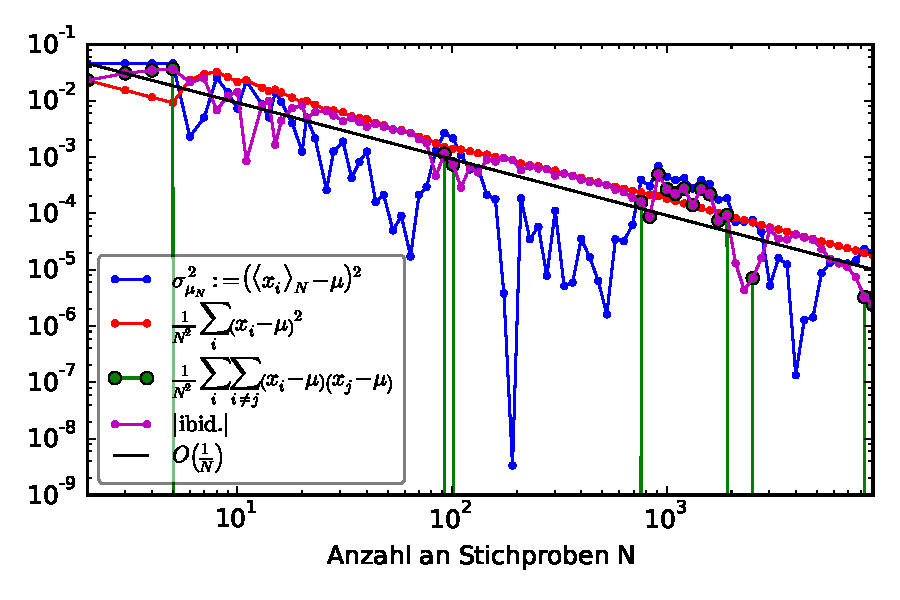
\includegraphics[width=\linewidth]{meanerror.pdf}
	\end{minipage}
	\caption{Darstellung der Standardvarianz des Mittelwertes $\sigma_{\mu_N}^2$ und der beiden in der Herleitung~\ref{eq:EabToEaEb-pre} auftretenden Summanden über die Anzahl einbezogener Stichproben. Hierbei ist zu beachten, dass beim Vergleich von den Werten für die Stichprobenanzahl von $N_1$ und $N_2$ die ersten $\min\left( N_1,N_2 \right)$ Stichproben identisch sind.}
	\label{fig:meanerrorsummand}
\end{figure}
